% Data flow diagram
% Author: David Fokkema
\documentclass{article}
\usepackage{tikz}
\usetikzlibrary{shapes,arrows}
\usepackage{pdflscape}
\usepackage[papersize={8.6cm, 3.4cm}, text={8.6cm, 4.3cm}]{geometry}
\usetikzlibrary{decorations.text}
\usepackage{xcolor}
% \selectcolormodel{gray}

\begin{document}
\thispagestyle{empty}
%\begin{landscape}
\begin{center}
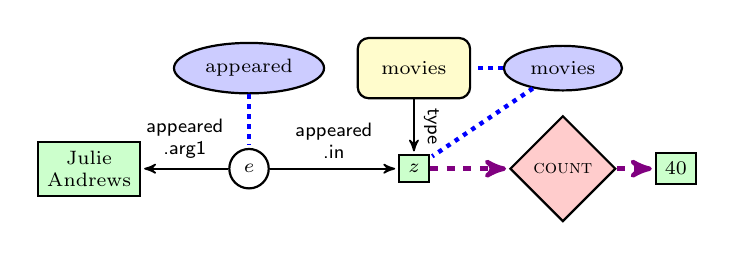
\begin{tikzpicture}[
  font=\sffamily,
  every matrix/.style={ampersand replacement=\&,column sep=0.4cm,row
sep=0.2cm,font=\scriptsize},
  entity/.style={draw,thick,rectangle,fill=green!20,font=\scriptsize},
  word/.style={draw,thick,ellipse,fill=blue!20},
  mediator/.style={draw,thick,circle},
  entityType/.style={draw,thick,rounded corners,fill=yellow!20,inner sep=.3cm},
  mathType/.style={draw,thick,diamond,fill=red!20,font=\scriptsize},
  mediatorToEntity/.style={->,>=stealth',shorten
>=1pt,semithick,black,sloped,above,font=\sffamily\scriptsize},
  typeToEntity/.style={->,>=stealth',shorten
>=1pt,semithick,black,sloped,above,font=\sffamily\scriptsize},
  wordToEntity/.style={-,>=stealth',shorten >=1pt,ultra
thick,dotted,blue,sloped,above,font=\sffamily\scriptsize},
  entityToMath/.style={->,>=stealth',shorten >=1pt,ultra
thick,dashed,violet,sloped,above,font=\sffamily\scriptsize},
  every node/.style={align=center}]

  % JulieAndrews has appeared in 40 movies .
  
  % Position the nodes using a matrix layout
  \matrix{ 
     \& \node[word] (wAppeared) {appeared}; \&
 \node[entityType] (tMovies) {movies}; \& \node[word] (wMovies) {movies}; 
\& \\
    \node[entity] (eAndrews) {Julie\\Andrews}; \& \node[mediator]
(mAppeared) {$e$}; \& \node[entity]
(eMovies)
{$z$}; \& \node[mathType][font=\sc\scriptsize] (mMovies) {count}; \&
\node[entity] (e40) {40};\\
  };
 
  % words to entities
  % \draw [wordToEntity] (wAndrews) edge node {}  (eAndrews);
  % \draw [wordToEntity] (w40) edge node {}  (e40);
  \draw [wordToEntity] (wMovies) edge node {}  (eMovies);
  % words to types
  \draw [wordToEntity] (wMovies) edge node {}  (tMovies);
  % event word to mediators
  \draw [wordToEntity] (wAppeared) edge node {}  (mAppeared);
  
  % mediator to entities
  \draw [mediatorToEntity] (mAppeared) edge node {appeared\\.arg1} 
(eAndrews);
  \draw [mediatorToEntity] (mAppeared) edge node {appeared\\.in} 
(eMovies);
  
  % types to entities
  \draw [typeToEntity] (tMovies) edge node {type}  (eMovies);
  
  % math func
  \draw [entityToMath] (eMovies) edge node {}  (mMovies);
  \draw [entityToMath] (mMovies) edge node {}  (e40);
 
\end{tikzpicture} 
 \scriptsize $\mbox{appeared.arg1}(e, \mathrm{Julie Andrews}) \wedge
\mbox{appeared.in}(e, z)$ \\ $\wedge\;
\mbox{movies}(z) \wedge \textsc{count}(z, 40)$
\end{center}


\end{document}